% !Mode:: "TeX:UTF-8"
\chapter{可行性分析与生存分析}
\label{cha:analyse}

\section{可行性分析}

\subsection{技术可行性}

通常对于生存分析与建立预后模型使用的是R语言,然后考虑到后期需要将训练得到的模型与后端进行组合,而且R语言的使用人数较少,没有完整的社区资源可供查询,而且为了减少最终系统的复杂度,最后使用了Python作为主要框架的语言。而Python中虽然官方包并没有支持生存分析与模型建立的内容,但是Python有大量第三方包可供调用。在Python中,可以使用的生存分析包的数量没有限制,只要这些包相互兼容,不造成冲突。如lifelines、scikit-survival、survival、pysurvival和scipy。每个包都有自己的优势和劣势,包的选择取决于分析的具体需要和目标。lifelines具有易于使用的API,用于常见的生存分析任务,如Kaplan-Meier估计、Cox比例危害回归和加速失败时间模型。支持随时间变化的协变量、左截断和区间删减。提供可视化工具,如生存曲线、危险函数和累积危险函数。虽然它对灵活的参数化生存模型和对竞争性风险分析的支持有限。但是在目前的标准下其已足够完成分析任务。而相比于lifelines,其他包比如scikit-survival相对于图形化的支持不足,而pysurvival由于复杂的语法和有限的文档,学习曲线可能很陡峭,scipy则ui较为简陋。所以最后选择了lifelines作为主要分析工具。

在后端方面,相比于Java的SpringBoot框架,Flask的环境要求相对较小,也比较容易编写相应的Dockerfile以满足简单的部署。同时考虑到和使用Python的模型结合,如果使用相同语言则可以直接将模型嵌入其中,所以最后使用了Flask作为主要框架。而笔者在大学期间与实习过程中已经积累了相应的在服务器、开发板中部署环境的经历。考虑到经济价格原因,最后的Flask项目先后在阿里云与树莓派开发板上完成过部署,已经确认Flask端的程序具有良好的部署性能与健壮性。而且Flask的良好接口文档也让这项工作有更多的资料可以参考学习。

在前端方面,本文使用的是Vue3作为框架,这里使用的是组合式API开发,相比于Vue2延续而来的选项式API,Vue3的结构更加清晰,使用了少缩进的组合展开方式,可以直接在setup中使用ref、watch等函数来分别管理变量和监控生命周期。这也为开发和后期更改提供了便利。

综上所述,通过分析患者生存情况训练预后模型,并开发使用Vue3-Flask的的管理系统具有技术可行性。

\subsection{其他可行性}

本系统成本主要包括软件开发成本、版权使用成本、硬件维护成本、数据收集成本。其中软件开发完全由笔者承担,除了占用的时间资源外不消耗其他费用。UI界面中使用的主要是Element-ui提供的图表等资源,MIT协议起源于麻省理工学院,是在所有软件许可中比较宽松的一种,授权人或使用者具有完全的使用、复制、更改、分发等等权力,所以使用相应的资源并不会消耗版权成本。硬件分别使用了阿里云和树莓派用来测试部署效果,阿里云仅仅使用了一个月,成本为12元,而树莓派在之前就已获取,在家运行成本忽略不计。数据来源分别来自SEER数据库与本地医院,SEER数据集中的数据较为完整,笔者通过提交申请后得到授权,随即即可访问相应软件并通过提取得到;而医院数据由于有关患者隐私具体细节不能公开,主要由数据库中进行笔者进行提取,而医院方面配合进行随访,最后由笔者与医院方面共同标记数据得到最后的测试数据。

综上所述,本文进行开发的资源和内容明确,经济成本在可负担范围内,同时使用的材料和内容都不侵犯相关法律条例或其他团体或个人权益,同时时间成本和开发技术栈都进行了有效的权衡,因此该项目可行性得证。

\section{需求分析}

\subsection{目标对象分析}

预后模型的主要面向对象是术后的子宫肉瘤患者和相关专业的医生与管理者,考虑到为了避免可能存在的恐慌和信息泄露,该模型及相关系统不会直接向患者或者大众开放,而是用于医疗数字化的应用,比如在医院内网或其他方面搭建。而考虑到使用对象是来自医院的医生、管理员以及后期维护人员,所以一个清晰的UI界面和所见即所得的管理面板是需要的,同时主要的两个用户角色也需要配备相应的权限管理与账户管理。同时为了方便管理员或后台维护人员进行后期的内容增广与技术更新,系统内部同样要配备一定的工单或消息处理与记录功能。从而能让各个角色都能迅捷而高效的完成各自所需要完成的工作。

另外,考虑到数据收集过程到最后模型中预测的不同,同时由于JavaScript到Flask中的表单信息和数据格式需要进行的变化。从前端到后端需要设计一个映射从而不影响数据的准确使用和训练。

\subsection{功能需求}

考虑到医院、医生多方面的需求,以及患者的实际需求,预后模型有以下几个功能或特点选项:
\begin{enumerate}
    \item 对于患者的预后数据,模型需要能够输入规定的所有患者数据,包括患者的年龄、肿瘤大小等,并根据这些数据进行推断
    \item 预后模型的输出要求可以有多种,比较常用的做法是单单对患者的三年或五年生存率进行判断,如果模型具有概率层,一个概率也将是可以选择的输出,可以用来描述该结果的准确度,以供医生了解结果的准确度。而在后文中,笔者将介绍一种新的方法,使用聚类来将患者分群,此时预后模型的输入相同,而输出则是患者的表征群。这个方法看似只评估了聚类的结果,结果没有之前的有意义。然而,实际上这个结果更加有统计学意义,因为相近的病情状况往往意味着病情的危险程度相近,所以这个结果也具有更好地判断有效性,对于临床使用的可行性也更好。
    \item 模型需要分析出各个输入因素的重要性,从而令模型有更好的解释性,对于树型模型需要有图显示其结构。
\end{enumerate}

而一体化平台则需要具有以下几个功能:
\begin{enumerate}
    \item 一个登录界面,用来进行基础的账号管理,登录时需要提供用户名与密码。后台存储的账号分别分为管理员与普通医生,需要hash加密密码以让用户登录更加安全,管理员具有访问更高级别页面的权限。考虑到信息安全问题不提供直接使用token或其他第三方机构账号登录。
    \item 系统首页,首页可以显示用户的头像和登录位置等信息,同时也显示当前用户上传的数据量与预测患者人数,通过对该功能的增广可以让管理员更方便地布置任务,显示其他信息等。
    \item 数据表格页面,数据表格可以显示按照上述规范的带标注的详细数据信息,数据实际信息在后台通过端口处理将接收到的文件按照映射表转换为csv格式的编码信息。这样的操作可以明显减少数据文件的体积,减少占用的内存。同时,数据表格页面同时提供了表单功能,从而方便医生录入新的数据并校验数据正确性。
    \item 工单记录功能,有关系统本身和待处理的信息都会在这个页面显示,符合权限要求或指定的接收用户能够在这个页面看到这个信息,而如果信息已经被读取则会标为已读。同时还提供了回收站功能来防止用户误删信息。
    \item 训练模型页面,训练模型页面提供了直接上传数据文件的功能,上传数据文件后,文件将通过js判断基础格式是否符合要求,如果符合就会被上传到后端中进行模型训练,训练完成后模型文件将会暂存在后端中,同时该页面下的数据表格也会显示当前的模型名称和评分等信息。如果选择不保存或删除模型,后端将会同时删除使用的表和模型文件。
    \item 预测数据页面同样提供了表格用来存储历史数据。用户可以选择使用的模型并通过直接填写页面中的表单并点击预测键即可预测患者的状况,为了方便起见,这里只选取了患者三年死亡与否的结果预后模型。在这里患者的详细信息被隐去,取而代之的是患者的三年生存与否和当前结果准确率的数据。这些历史记录同样有删除功能
    \item 权限管理页面,权限管理页面提供了上述各页面的权限更改功能。其中只有管理员可以修改用户角色,而也只有管理员可以添加新的角色并赋予给用户。管理员可以给用户角色设置对每个页面能否访问。
\end{enumerate}

\section{变量选择}

在研究过程中,笔者首先阅读了一些有关子宫肉瘤列线图与模型相关的文章\cite{novel_tool},在这些文章中,年龄、种族、地区、婚姻状况、肿瘤大小、淋巴结状态、分期、分级、化疗、放疗都是比较常用的数据。然后在对SEER的数据集进行筛选后,我发现主要的库中婚姻状况等参数由于隐私原因被移除,而淋巴结的信息符合标准的过少,如果使用则会大大削减符合要求的数据数量,从而让训练集变得很小,所以考虑到这点后没有纳入。与医院老师们沟通后,笔者发现分期中的一些描述包含了淋巴结是否被侵犯的状况,而目前医院内主要使用化疗作为主要手段,放疗的数据较少所以没有考虑纳入,所以最后选择了选择了当前的变量。

\section{生存分析}

\subsection{数据概况}

从SEER数据集中采集到的数据一共有62470条,患者的年龄分布如下图所示:
\begin{figure}[!htbp]
    \centering
    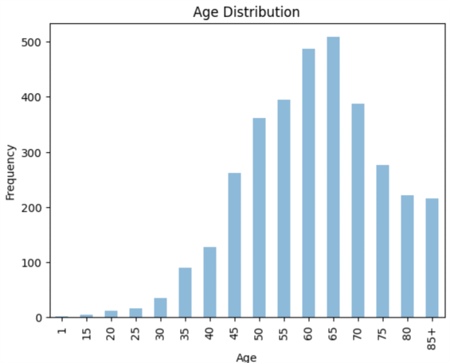
\includegraphics[scale=0.8]{age_distribution.png}
    \caption{SEER数据集中患者年龄分布图} \label{fig:age_distribution}
\end{figure}

由于基数较大,同时表格中的数值取区间中的最低值,表中的频数对其进行了平均缩减以方便显示,可以看到表格中用户的年龄主要集中在60-70之间,这说明了患者的年龄越大,越有可能患子宫肉瘤,如果按照三分位数进行划分,我们可以得到子宫肉瘤的主要发病人群集中在45岁到65岁之间。

而对于另外一个数值变量,肿瘤大小的分布如下图所示:

\begin{figure}[!htbp]
    \centering
    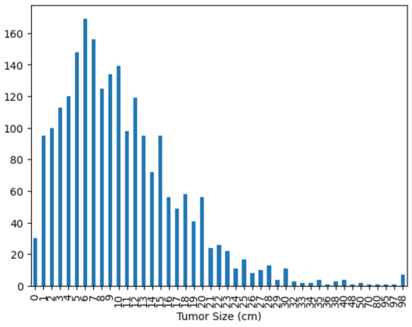
\includegraphics[scale=0.8]{tumor_size_distribution.png}
    \caption{SEER数据集中患者肿瘤大小分布图} \label{fig:tumor_size_distribution}
\end{figure}

按照上述表格同样可以得到肿瘤大小的大致分布,肿瘤大小的中间值在50mm左右,肿瘤大小为0mm代表1mm以下或较难以衡量的数据,而肿瘤大小在到达50mm的峰值后则呈反曲线状态减少,直到到达最低点。肿瘤大小的分布较为复杂,因为这个原因所以我们也很难为其划分一个清晰的界限来划分患者,如果直接划分很可能会损失一部分信息。这里先使用50mm为分界点进行划分,后期再是用其他方法进行比较。

\subsection{Kaplan-Meier曲线绘制}

由于下面使用的Cox比例风险模型需要数据满足以下假设:
\begin{enumerate}
    \item 风险比值的对数与协变量之间呈线性关系
    \item 风险比值的对数与时间无关
\end{enumerate}

上面的风险比值的对数与协变量之间呈线性关系假设需要使用Kaplan-Meier曲线进行验证。具体方法是:对于同一自变量,如果本身为分类型变量直接使用,如果为连续或数值型变量,则把变量分为多个区间作为不同值,观察曲线间状态,如果曲线存在交叉则说明其不满足假设,反之则说明风险比值和协变量间存在线性关系,满足条件。

同时,KM曲线不但可以验证后续的假设是否成立,同时也能对患者的生存状况做更细致的分析。KM曲线的原理是首先计算在某一时期存活的病人能活到下一时期的概率,然后将存活概率逐一相乘,得到相应时期的存活率。这种方法可以非常清晰地看到两组患者在不同时间的生存率差异。

由于篇幅问题,这里仅列举两张比较典型的进行分析说明:

\begin{figure}[!htbp]
    \centering
    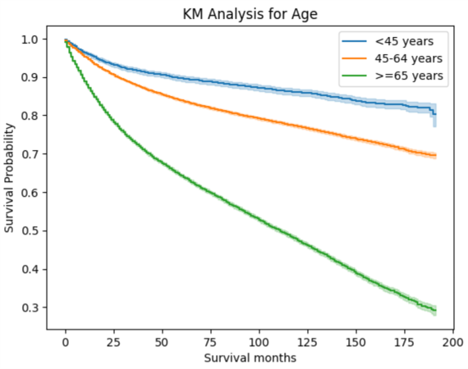
\includegraphics[scale=0.8]{km_age.png}
    \caption{SEER数据集中患者年龄KM曲线图} \label{fig:km_age}
\end{figure}

从图\ref{fig:km_age}中可以看到,45岁以下的患者在时间变化下衰减最少,而45-64的次之,65以上减少最快,而这些曲线都不交叉,置信区间也较小。这说明了患者的年龄是一个重要影响因素,而患者的年龄越小,生存率越高。

\begin{figure}[!htbp]
    \centering
    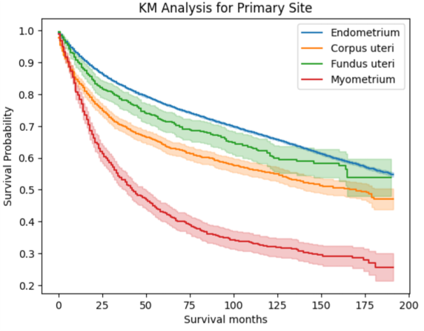
\includegraphics[scale=0.8]{km_site.png}
    \caption{SEER数据集中患者原发部位KM曲线图} \label{fig:km_site}
\end{figure}

从图\ref{fig:km_site}中可以看到,四个原发部位的患者生存率从高到低的变化,从置信区间的的范围可以看到四者的数据量也存在差异。同时这些组间也存在线性比例关系,所以满足假设。

\subsection{Cox单因素分析}

Cox单因素分析是一种基于Cox比例风险模型的统计分析方法,它可以用于研究变量对于结果的影响。本文使用年龄、种族、原发部位、肿瘤大小、分期、化疗情况、分级建立Cox模型,并使用SEER数据集中的数据编码为合适格式,用编码后的结果训练。下列的表\ref{tab:cox_univar}是单因素模型的Cox分析结果。

\begin{table}[htb]
    \centering
    \begin{minipage}[t]{0.8\linewidth} 
    \caption[预测子宫肉瘤患者总生存率的单变量Cox分析]{预测子宫肉瘤患者总生存率的单变量Cox分析}
    \label{tab:cox_univar}
      \begin{tabularx}{\linewidth}{lXX}
        \toprule[1.5pt]
        {\heiti variable} & {\heiti exp(coef)} & {\heiti P value} \\\midrule[1pt]
        \textbf{Age} \\
        \textless45years \\
        45-64years & 1.68 & \textless0.005 \\
        $ \geq $65years & 4.35 & \textless0.005 \\\midrule[1pt]
        \textbf{Race} \\
        White \\
        Black & 0.56 & \textless0.005 \\
        Asian or Pacific Islander & 0.47 & \textless0.005 \\\midrule[1pt]
        \textbf{Primary Site} \\
        C54.1-Endometrium \\
        C54.9-Corpus uteri & 1.67 & \textless0.005 \\
        C54.3-Fundus uteri & 1.43 & \textless0.005 \\
        C54.2-Myometrium & 3.24 & \textless0.005 \\\midrule[1pt]
        \textbf{Tumor Size} \\
        \textless50mm \\
        $ \geq $50mm & 2.36 & \textless0.005 \\\midrule[1pt]
        \textbf{Stage} \\
        Localized \\
        Regional & 2.72 & \textless0.005 \\
        Distant & 10.94 & \textless0.005 \\\midrule[1pt]
        \textbf{Chemotherapy} \\
        Yes \\
        No/Unknown & 0.41 & \textless0.005 \\\midrule[1pt]
        \textbf{Grade} \\
        Well differentiated; Grade I \\
        Moderately differentiated; Grade II & 1.84 & \textless0.005 \\
        Poorly differentiated; Grade III & 4.93 & \textless0.005 \\
        Undifferentiated; anaplastic; Grade IV & 6.95 & \textless0.005 \\
        \bottomrule[1.5pt]
      \end{tabularx}
    \end{minipage}
  \end{table}

coef是Cox中的回归系数beta,因此exp(coef)是Cox比例风险模型中的概率风险比。从结果中可以看到,计算得到的P值是用来评估同一变量的协变量对因变量的影响是否显著的参数。这里使用变量中的第一个协变量作为参照,分析其他协变量是与对照变量存在显著差异。一般在0.05以下则说明变量对于结果的影响较为显著,可以看到表中的结果都在该值之下,所以说明每个变量的不同值对于计算结果的影响较为显著,同时也验证了在Kaplan-Meier曲线中观察到的结果。

\subsection{Cox多因素分析}

Cox多因素分析也是一种基于Cox比例风险模型的统计分析方法,它可以用于研究多个不同的变量对于结果的影响。下列模型同样使用年龄、种族、原发部位、肿瘤大小、分期、化疗情况、分级建立Cox模型,并使用SEER数据集中的数据编码为合适格式,用编码后的结果训练。不同的是单因素将变量的每个值作为参数导入,而且同时只导入一个变量,而多因素分析则直接导入有不同值e多个变量。下列的表\ref{tab:cox_multivar}是多因素模型的Cox分析结果。

\begin{table}[htb]
    \centering
    \begin{minipage}[t]{0.8\linewidth} 
    \caption[预测子宫肉瘤患者总生存率的多变量Cox分析]{预测子宫肉瘤患者总生存率的多变量Cox分析}
    \label{tab:cox_multivar}
      \begin{tabularx}{\linewidth}{lXX}
        \toprule[1.5pt]
        {\heiti variable} & {\heiti exp(coef)} & {\heiti P value} \\\midrule[1pt]
        \textbf{Age} & 2.23 & \textless0.005 \\
        \textbf{Race} & 0.82 & \textless0.005 \\
        \textbf{Primary Site} & 1.17 & \textless0.005 \\
        \textbf{Tumor Size} & 1.52 & \textless0.005 \\
        \textbf{Stage} & 2.47 & \textless0.005 \\
        \textbf{Chemotherapy} & 1.29 & \textless0.005 \\
        \textbf{Grade} & 1.56 & \textless0.005 \\
        \bottomrule[1.5pt]
      \end{tabularx}
    \end{minipage}
  \end{table}

从结果中可以看到,计算得到的P值是用来评估多个变量对因变量的影响是否显著的参数。这里由于不是同一变量,所以不需要像单变量分析一样使用变量中的第一个协变量作为参照,分析其他协变量是与对照变量存在显著差异,相反,由于多个变量互不交叉,其是并不需要设置一个变量作为参照组。一般在0.05以下则说明变量对于结果的影响较为显著,可以看到表中的结果都在该值之下,所以说明每个变量对于计算结果的影响较为显著。这是在Kaplan-Meier曲线阶段无法观察到的多变量影响,这说明不但单个变量的不同值对于结果有比较大的影响,同时这个结果也可以在多变量模型中观察到,进一步验证了所选取的变量都有纳入价值。

\subsection{生存分析结论}

在上述对于患者数据库内数据分布的分析后,本文分别进行了Kaplan-Meier曲线的绘制和Cox单变量和多变量分析。其中对于数据的分布分析让我们对于数据库中的人群特征有了一定的了解,同时也为如何对变量类型为数值变量的变量进行了一定的划分,从而方便后续在Cox模型中导入并训练。而Kaplan-Meier曲线的绘制有两个目的,第一个目的是可以初步对于不同变量对结果的影响,从而让我们能够初步对于是否纳入该变量有一定的预判,在之前的工作中,笔者对于如何纳入变量有了较多考量,其中首先从论文中选择了一些常用的、对结果影响较大的变量,同时也选择了一些其他的未纳入过的变量,而这些变量中的一部分便因为KM曲线结果不符合模型标准或在这之前便发现变量内容与其他变量具有重复或冲突,所以最后没有纳入。而如果在这个阶段提前使用Kaplan-Meier曲线进行分析的话可能就能避免之前的重复劳动。Cox单因素模型分析选择了每个变量的不同值,将它们进行了拆分为二元变量并堆叠为组的过程,从而导入Cox单因素模型进行分析,在这个过程中,可以得到之前使用Kaplan-Meier曲线不能看到的的精确数值表示,这样便可以让我们对于数据是否能够纳入得到一个更明确地标准,而不是对于曲线进行经验判断。而多因素分析则解构了多个变量,分期它们结合起来对于结果的影响是否显著,这里与之前不同,如果只有单个变量只需要使用 log-rank 检验来确定因素之间的显著性关系即可,而多变量则需要使用比例风险回归模型才能确认影响,如果某一变量在 log-rank 检验中显示影响较大,在多变量回归中可能会因为其他变量占比较大从而反而显示不出较好的影响。而当前结果表明,目前采用的变量都对于结果有较为显著的影响,在之后的模型纳入与训练中可以作为参数使用。